\chapter[Materiais e métodos]{Materiais e métodos}

\hl{ADICIONAR DESC. INICIAL}

\section{O dado} \label{sec:dataset}

Como dito, existem diversos tipos de áreas de desenvolvimento que caracterizam a Inteligência Artificial. A área de \textit{machine learning} é caracterizada pela capacidade da máquina aprender a partir de experiências com o dado, por isso deve-se dar uma enorme importância para a qualidade do dado para conseguir resolver problemas com ML, mais ainda para \textit{Deep Learning}. Para ser possível a construção de um modelo que visa testar a hipótese de estudo em questão, seria necessário realizar o levantamento de um conjunto de dados em formato de texto, em português, que fosse possível alimentar o modelo a ser criado.

O Grupo de Pesquisa em Aprendizado de Máquina (GPAM) da Universidade de Brasília desenvolveu em 2018 um projeto de pesquisa que visa realizar a classificação das repercussões gerais do Supremo Tribunal Federal (STF) \cite{cnn-for-STF}. Para essa classificação, o projeto precisava realizar a extração de informações dos textos das decisões judiciais do STF, sendo essas possuindo documentos digitais tanto formulados digitalmente, manuscritos e/ou escaneados. Tal conjunto de dados foi fornecido para o presente trabalho de conclusão a fim de facilitar o processo de aquisição dos mesmos por meio de \textit{crawlers}\footnote{
  \textit{Crawlers} ou \textit{web crawlers} são tecnologias que possibilitam a extração de informações disponíveis em sites da Internet de maneira organizada para possibilitar o consumo desses dados para desenvolvimento de algoritmos. Bastante comum para criação de base de dados de ML.
} ou outras fontes.

\subsection{Características}

Foram fornecidos 89.578 processos do Supremo Tribunal Federal em formato PDF, contendo os diversos temas de repercussões gerais e diferentes características \cite{cnn-for-STF}. Algumas delas são:

\begin{itemize}
  \item O STF recebe processos em segunda instância de todo o Brasil e não existe nenhum padrão em sua formatação, fonte, espaçamento e escrita;
  \item Uma parte significante dos documentos fornecidos estão em forma de imagem obtidas por meio de \textit{scanners} e muitas vezes possui anotações, estampas, marcas d'agua, manchas, sombras, etc.
\end{itemize}


No projeto desenvolvido, o GPAM realizou um conjunto de extrações e formatações dos documentos para facilitar o trabalho a partir de uma etapa de processamento.

\begin{figure}[H]
  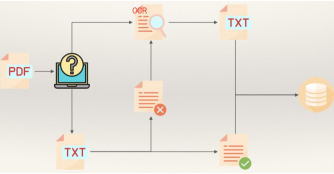
\includegraphics[width=13cm, center]{figuras/gpan-pipeline.png}
  \caption{Fluxo de processamento de processos do STF pelo GPAM.}
  \label{fig:gpan-pipeline}
\end{figure}

Nesse processamento, uma das etapas consistiu em verificar se a página do documento possui texto selecionável ou não, para então realizar a extração do texto via algoritmo de OCR. Tudo isso foi armazenado em um arquivo CSV, cuja as principais estão descritas a seguir.

% process_id,,,,,document_id,,,page_is_ocr,,page_text_extract,page_number,,

\begin{table}[h]
 \centering
 \caption{Principais características do dado CSV}
 \begin{tabular}{|m{9em}|m{20em}|}
    \hline
      \textbf{Coluna}  &
      \textbf{Descrição} \\
    \hline
      \textit{process\_id}  &
      Parte do número do processo no tribunal \\
    \hline
      \textit{document\_id}  &
      Identificador do documento dentro do processo \\
    \hline
      \textit{page\_is\_ocr}  &
      Booleano definindo se a página necessita de OCR \\
    \hline
      \textit{page\_text\_extract} &
      Texto extraído da página utilizando OCR \\
    \hline
      \textit{page\_number} &
      Número da página do PDF a qual aquela extração pertence \\
    \hline
 \end{tabular}
 \label{tab:csv-details}
\end{table}

É importante notar que os campos \textit{process\_id} e \textit{document\_id} se repetem no CSV mas a junção de ambos juntamente com a \textit{page\_number} identificam unicamente a página dentro do PDF.

\subsection{Tratamento e formação do \textit{dataset}}

Por se tratar de uma problemática diferente do GPAM, foi preciso consumir o que foi fornecido e gerar novos dados que se encaixem melhor para a solução. Para tal, criou-se um conjunto de algoritmos para pegar os dados e realizar essa adequação no formato de uma \textit{pipeline}\footnote{
  Na computação, o termo \textit{pipeline} define um conjunto de processamentos de dados conectados em série, onde a saída de um desses elementos de processamento é a entrada do próximo, sendo elas dependentes para o processamento ser executado adequadamente.
}, com etapas de separação de documentos que possuem páginas que necessitam de OCR, extração de imagem a partir de PDF, criação de filtros de imagem e extração de informação de imagem utilizando o OCR.

\begin{figure}[H]
  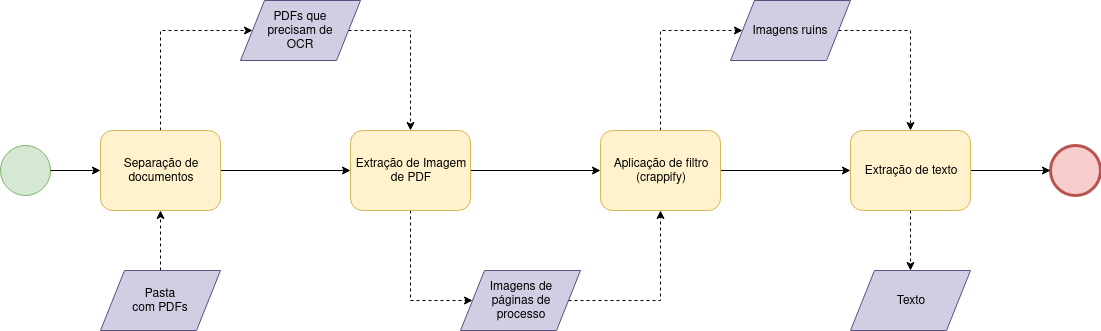
\includegraphics[width=\linewidth, rotate=0, center]{figuras/crappy-flow-diagram.png}
  \caption{Processo para a criação de \textit{dataset}.}
\end{figure}

\subsubsection{Separação de documentos}
O conjunto de PDFs fornecidos como dados estavam todos juntos em um único diretório no disco, sem a correta divisão de qual era o dado contido no PDF. O CSV fornecido pelo GPAN e os itens descritos na tabela \ref{tab:csv-details} fazem referência a todas as páginas desses PDFs e possui também o seu conteúdo, sendo eles extraídos por meio de OCR ou não, como mostra a figura \ref{fig:gpan-pipeline}. Porém como o foco do trabalho é realizar estudos sobre a qualidade do OCR, decidiu-se por separar o dado entre os que foram extraídos utilizando OCR dos que não foram.

Para isso, gerou-se um novo CSV apenas com os registros de páginas cujo necessitou-se do OCR em sua extração e criou-se também um diretório para armazenar apenas os PDFs que possuíam páginas não-selecionáveis. Dos 89.578 arquivos, existem cerca de 354.501 páginas somadas, sendo essas:

\begin{table}[H]
  \centering
  \caption{Divisão de páginas dos PDFs.}
  \begin{tabular}{|m{10em}|c|}
    \hline
      \textbf{Tipo}  &
      \textbf{Quantidade} \\
    \hline
      Necessita de OCR  &
      80.624 \\
    \hline
      Não necessita de OCR  &
      273.877 \\
    \hline
      \textbf{TOTAL}  &
      \textbf{354.501} \\
    \hline
  \end{tabular}
  \label{tab:csv-diff}
\end{table}

\subsubsection{Extração de imagem do PDF}
Com os dados separados em um diretório específico, iniciou-se a etapa de extração de imagem a partir dos documentos em formato PDF dos processos. Utilizou-se também informações do CSV (tabela \ref{tab:csv-details}) para selecionar a página específica do documento a qual o OCR foi utilizado, diminuindo assim o tempo de processamento por documento.

A extração de imagem a partir do PDF é feita utilizando um algoritmo de software livre desenvolvido em Python, chamado de \textit{pdf2image}. Ele recebe como entrada um PDF e é possível definir qual ou quais páginas do PDF deseja-se extrair, permitindo assim a geração do \textit{dataset} de imagens de processos.

\subsubsection{Aplicação de filtros}
Para a criação de um modelo generativo que consiga diminuir os ruídos de imagens, é preciso utilizar como dado de entrada imagens que possuam tais características - ruídos. Das 354 mil páginas dos PDFs disponíveis, fazer a separação de todas elas para a identificação de imagens ruins deria um trabalho bem complexo e que diminuiria o tempo disponível para o desenvolvimento do presente trabalho. Com isso, adotou-se a heurística de que todas as fotos que tiveram texto extraído via OCR (tabela \ref{tab:csv-diff}) seriam "pioradas" aplicando um conjunto de filtro de imagens de diferentes tipos.

Um filtro de imagem é um algoritmo ou rotina de software que consegue alterar de forma fixa ou aleatória os valores dos pixels contidos em uma imagem. Com isso, é possível criar uma lógica que tente simular imagens escaneadas de maneira automatizada, aplicando sombreamento, borrões, manchas, distorções, etc.


\begin{figure}[H]
  \centering
  \begin{subfigure}{.5\textwidth}
    \centering
    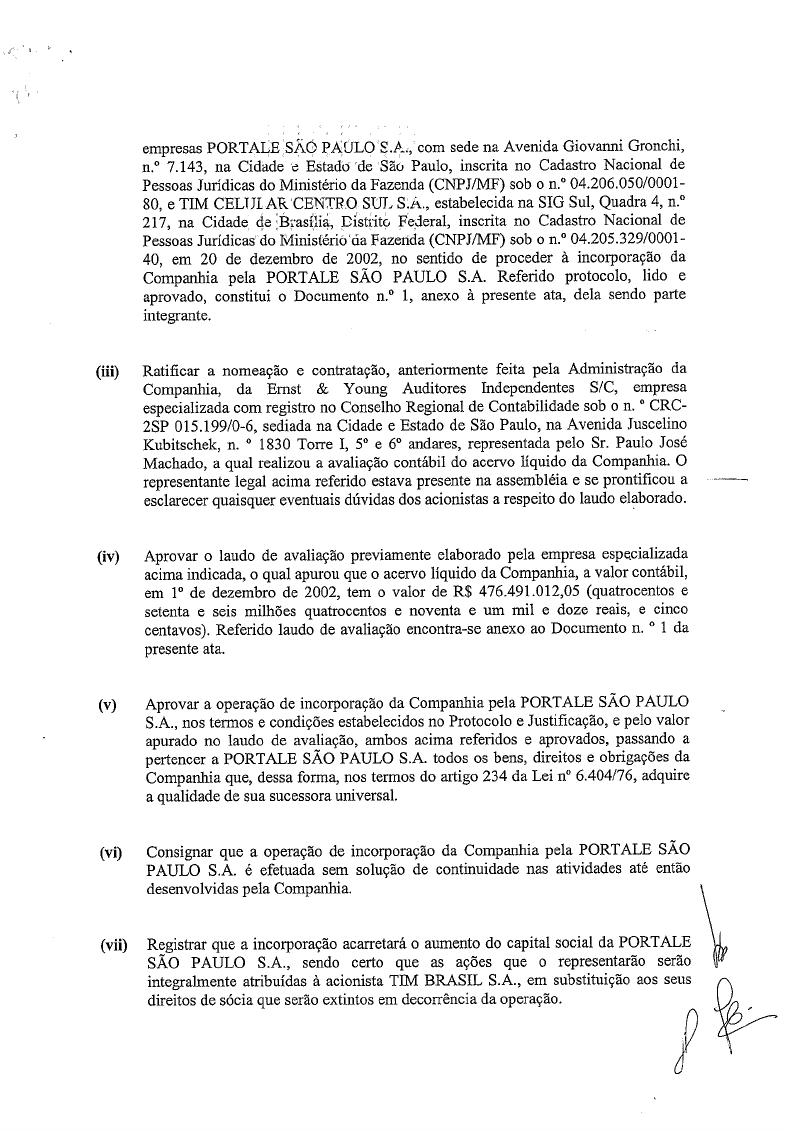
\includegraphics[width=0.8\linewidth]{figuras/good-text-image.jpg}
    \caption{Foto sem filtro}
    \label{fig:image-without-filter}
  \end{subfigure}%
  \begin{subfigure}{.5\textwidth}
    \centering
    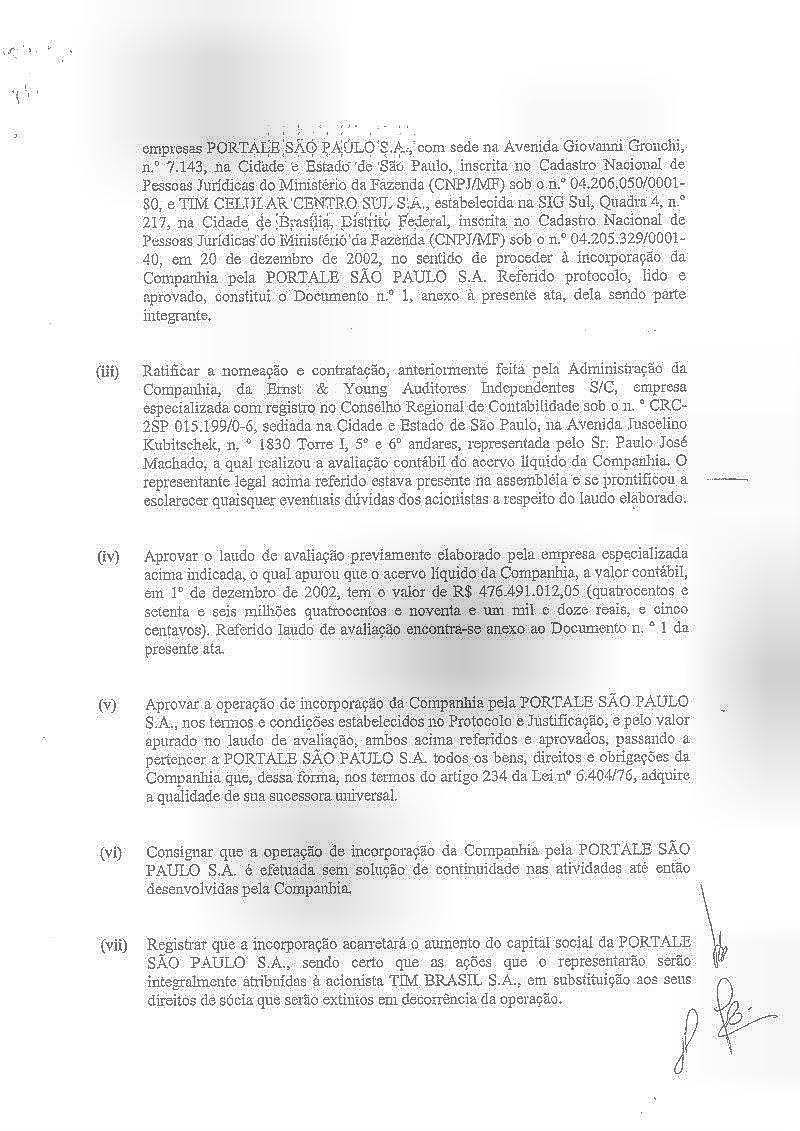
\includegraphics[width=0.8\linewidth]{figuras/image-with-overlay.jpg}
    \caption{Foto com filtro aplicado}
    \label{fig:image-with-filter}
  \end{subfigure}
  \caption{A figure with two subfigures}
  \label{fig:side-process-images}
\end{figure}

Existem diversas bibliotecas já implementadas em Python que possibilitam a aplicação de filtros em imagens. As utilizadas foram: \textit{ImageFilter} da biblioteca \textit{Python Imaging Library} e \textit{imgaug}, biblioteca de \textit{data augmentation}\footnote{
  Processo de transformação do dado que permite que seu tamanho cresca, fornecendo assim mais insumos ou entradas de dados disponíveis em um processo de treinamento.
}. Alguns filtros foram de origem autoral.

Abaixo, listam-se todos os filtros utilizados e estudados para o presente processamento de imagem.

\begin{table}[H]
  \centering
  \caption{Descrição dos filtros utilizadosverbo tesselar.}
  \begin{tabular}{|m{.25\linewidth}|m{.1\linewidth}|m{.55\linewidth}|}
    \hline
      \textbf{Nome}  &
      \textbf{Fonte}  &
      \textbf{Descrição} \\
    \hline
      EDGE\_ENHANCE  &
      PIL  &
      Aumenta o contraste dos píxels ao redor de bordas para que essas bordas se destaquem mais do que os demais elementos da foto  \\
    \hline
      CONTOUR  &
      PIL  &
      Similar ao EDGE\_ENHANCE mas com maior intensidade \\
    \hline
      RandomOverlay  &
      autoral  &
      Cria formas gerométricas randômicas e transparentes e as coloca acima da imagem original, dando a impressão de manchas. A posição das formas também é randômica. \\
    \hline
      PerspectiveTransform  &
      \textit{imgaug}  &
      Aplica randomicamente transformações de 4 pontos de perspectiva, dando uma ideia de "lupa" para algus pontos da imagem \\
    \hline
      SaltAndPepper  &
      \textit{imgaug}  &
      Substitui píxels randômicos da imagem por píxel de sal (cor branca) e pimenta (cor preta) \\
    \hline
      GammaContrast  &
      \textit{imgaug}  &
      Ajusta o contraste da imagem escalando os píxels da imagem em um valor calculado por \(x = 255(\frac{v}{255})^{\gamma}\), onde $\gamma$ é um parâmetro da função entre $0$ a $1$ e $v$ é o antigo valor do píxel \\
    \hline
      JpegCompression  &
      \textit{imgaug}  &
      Degrada a imagem aplicando uma compressão de JPEG, diminuindo sua qualidade \\
    \hline
      Dropout  &
      \textit{imgaug}  &
      Randomicamente coloca uma fração de pixels da imagem para o valor 0 \\
    \hline
      Affine  &
      \textit{imgaug}  &
      Aplica transformações na imagem mas mantém relações de colinearidade e distância. Geralmente composta por rotações, translações e dilatações das formas presentes na imagem. \\
    \hline
  \end{tabular}
  \label{tab:sdas}
\end{table}

As tecnologias de OCR disponíveis, como o Tesseract, em geral são muito sensíveis e aplicar todos esses filtros em uma única imagem impede que o OCR identifique caracteres nas mesmas. Com isso, é preciso escolher randomicamente entre os filtro listados, podendo aplicar um ou mais deles, mas nunca podendo aplicar todos de uma só vez.

O processo seguido para a criação de imagens ruins foi de que, para cada uma imagem boa, gera-se uma imagem ruim. Isso se dá pela alta quantidade de imagens disponíveis para treinamento, visto que se for necessário o consumo de mais imagens para treinamento na etapa de geração do modelo, é possível utilizar de \textit{data augmentation} para ampliar a base de dados.

\begin{figure}[H]
  \centering
  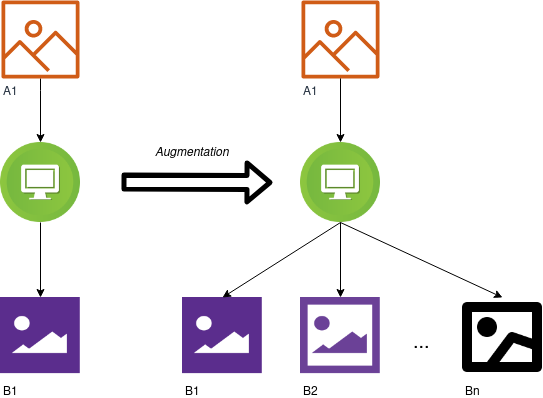
\includegraphics[scale=.6]{figuras/data-augmentation.png}
  \caption{Geração de imagens atual vs geração com \textit{data augmentation}}
  \label{fig:data-augmentation}
\end{figure}

\subsubsection{Extração de texto via OCR}

Para a extração de caracteres utilizando o OCR, fez-se o uso da tecnologia desenvolvida Tesseract, que atualmente conegue identificar e reconhecer mais de 100 idiomas por meio da configuração \textit{unicode}\footnote{
  Padrão que permite que os sistemas informatizados representem e manipulem textos de quaisquer idiomas de escrita que existem na atualidade. Fonte: Wikipedia.
}. Para tal, configura-se o Tesseract com a extensão para a lingua portuguesa, já disponível pela comunidade para uso.

Todo o texto extraído é armazenado em um CSV de saída que identifica qual o processo, documento e página que a extração foi feita. Isso depois servirá como base para a verificação e métrica para a comparação entre o texto extraído de uma página limpa para uma página com ruídos.

\section{Método proposto}

Para a criação de qualquer projeto científico deve-se seguir ou criar um método de trabalho que possibilite a construção de uma solução que consiga mostrar, de maneira clara e objetiva, o trabalho realizado para a comprovação, validação ou invalidação da hipótese apresentada.

Portanto, no presente projeto desenvolveu-se uma metodologia que possibilite validar se um modelo gerador de ML consegue melhorar a qualidade do OCR de fotos ruins. Tal método é dividido em 4 (quatro) grandes frentes que vão desde trabalho e curadoria do dado até a análise de métricas de qualidade de OCR. Essas frentes são: geração de \textit{dataset}, extração de OCR de imagens ruins, gerador de imagens e métricas de qualidade de OCR. As duas primeiras delas foram anteriormente detalhadas na sessão \ref{sec:dataset}. As duas etapas finais e não menos importantes serão detalhadas na sequência.

\subsection{Gerador de Imagens}

Essa etapa consistem em desenvolver um modelo de IA que receba como entrada uma imagem ruim e gere uma nova imagem nunca vista antes. Essa imagem é gerada a partir de uma Rede Neural Convolucional, como já foi citado em capítulos anteriores \hl{REFERENCIAR GENERATIVO}.

\hl{COLOCAR IMAGEM SIMULANDO O GENERATIVO}

Tendo uma nova imagem gerada e todas as informações necessárias identificadas previamente, como OCR das imagens boas e ruins, adiciona-se uma camada de extração de texto das imagens geradas pelo modelo Gerador e as adiciona no CSV contendo as extrações anteriores. Com isso, tem-se agora o insumo necessário para a criação de uma métrica de validação da hipótese.

\subsection{Métrica de qualidade do OCR}

Basicamente, para se conseguir alcançar o objetivo proposto do presente trabalho, seria necessário ter extrações de OCR de uma imagem boa, uma imagem ruim e de uma imagem nunca antes vista, gerada pelo modelo de IA. Com todas as etapas anteriores a essa realizando as devidas ações, permite-se então que as métricas de qualidade do OCR dos modelos gerados sejam extraídas, visto que as informações estão disponíveis.

Para a extração de informação de uma imagem utilizando OCR, primeiro realiza-se um processo de segmentação na imagem para a identificação de áreas onde o texto se encontra. A partir dessa segmentação, extrai-se o texto daquela região segmentada em especifico \cite{metrics-for-ocr-performance}, permitindo então que o processo de reconhecimento das informações possa ser extraído por caracter, palavra ou linha.

Porém, o processo de sementação da imagem pode ser o responsável pelo impedimento ou pela má qualidade da identificação do OCR. Esse tipo de erro pode ser uma separação (do inglês \textit{split}) ou mesclagem (do inglês \textit{merge}), tanto entre palavras de uma linha (horizontal) quanto entre duas linhas (horizontal), o que caracterizam 4 tipos de erros de segmentação \cite{metrics-for-ocr-performance}, sendo eles:
\begin{itemize}
  \item Mesclagem horizontal (HM)
  \item Separação horizontal (HS)
  \item Mesclagem vertical (VM)
  \item Separação vertical (VS)
\end{itemize}

\begin{figure}[H]
  \centering
  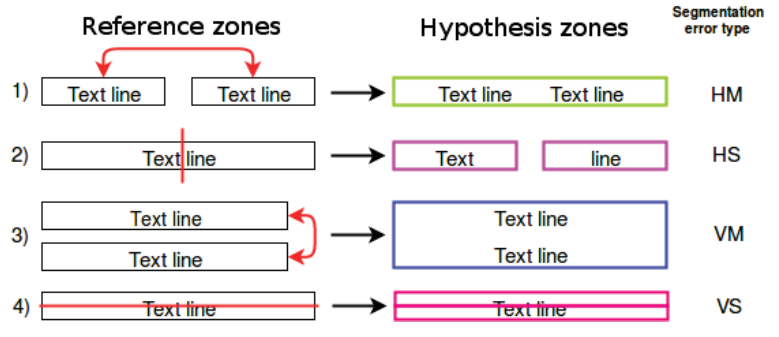
\includegraphics[scale=0.55]{figuras/ocr-segmentation-error.png}
  \caption{Tipos de erros de segmentação de imagem para apliações de OCR.}
\end{figure}